% `template.tex', a bare-bones example employing the AIAA class.
%
% For a more advanced example that makes use of several third-party
% LaTeX packages, see `advanced_example.tex', but please read the
% Known Problems section of the users manual first.
%
% Typical processing for PostScript (PS) output:
%
%  latex template
%  latex template   (repeat as needed to resolve references)
%
%  xdvi template    (onscreen draft display)
%  dvips template   (postscript)
%  gv template.ps   (onscreen display)
%  lpr template.ps  (hardcopy)
%
% With the above, only Encapsulated PostScript (EPS) images can be used.
%
% Typical processing for Portable Document Format (PDF) output:
%
%  pdflatex template
%  pdflatex template      (repeat as needed to resolve references)
%
%  acroread template.pdf  (onscreen display)
%
% If you have EPS figures, you will need to use the epstopdf script
% to convert them to PDF because PDF is a limmited subset of EPS.
% pdflatex accepts a variety of other image formats such as JPG, TIF,
% PNG, and so forth -- check the documentation for your version.
%
% If you do *not* specify suffixes when using the graphicx package's
% \includegraphics command, latex and pdflatex will automatically select
% the appropriate figure format from those available.  This allows you
% to produce PS and PDF output from the same LaTeX source file.
%
% To generate a large format (e.g., 11"x17") PostScript copy for editing
% purposes, use
%
%  dvips -x 1467 -O -0.65in,0.85in -t tabloid template
%
% For further details and support, read the Users Manual, aiaa.pdf.


% Try to reduce the number of latex support calls from people who
% don't read the included documentation.
%
\typeout{}\typeout{If latex fails to find aiaa-tc, read the README file!}
%


\documentclass[]{aiaa-tc}% insert '[draft]' option to show overfull boxes

 \usepackage{varioref}%  smart page, figure, table, and equation referencing
 \usepackage{wrapfig}%   wrap figures/tables in text (i.e., Di Vinci style)
 \usepackage{threeparttable}% tables with footnotes
 \usepackage{dcolumn}%   decimal-aligned tabular math columns
  \newcolumntype{d}{D{.}{.}{-1}}
 \usepackage{nomencl}%   nomenclature generation via makeindex
  \makeglossary
 % \usepackage{subfigure}% subcaptions for subfigures
 % \usepackage{subfigmat}% matrices of similar subfigures, aka small mulitples
 \usepackage{subcaption}
 \usepackage{fancyvrb}%  extended verbatim environments
  \fvset{fontsize=\footnotesize,xleftmargin=2em}
 \usepackage{lettrine}%  dropped capital letter at beginning of paragraph
 \usepackage[colorlinks]{hyperref}%  hyperlinks [must be loaded after dropping]

 \title{Passive Haptics to Enhance Virtual Reality Simulations}

 \author{Richard Joyce\thanks{Ph. D. Candidate, Mechanical and Aerospace Engineering, Student Member AIAA.}
  \ and Stephen K. Robinson\thanks{Director – UC Davis Center for Human/Robotics/Vehicle Integration and Performance, Professor – Mechanical and Aerospace Engineering, Member AIAA.}\\
  {\normalsize\itshape University of California, Davis, Davis, CA 95616}\\
 }

 % Data used by 'handcarry' option if invoked
 \AIAApapernumber{YEAR-NUMBER}
 \AIAAconference{Modeling and Simulation Technologies Conference, January 2017, Dallas, TX}
 \AIAAcopyright{\AIAAcopyrightD{YEAR}}

 % Define commands to assure consistent treatment throughout document
 \newcommand{\eqnref}[1]{(\ref{#1})}
 \newcommand{\class}[1]{\texttt{#1}}
 \newcommand{\package}[1]{\texttt{#1}}
 \newcommand{\file}[1]{\texttt{#1}}
 \newcommand{\BibTeX}{\textsc{Bib}\TeX}

\begin{document}

\maketitle

\begin{abstract}
% \lettrine[nindent=0pt]{R}{ecent}
Recent advances in virtual reality technology have renewed interest in the use of head-mounted display based aerospace simulation.
We present work on a virtual reality system that combines low fidelity physical prototypes, providing what is commonly called ``passive haptics'', with high fidelity visuals provided by a virtual reality head-mounted display.
Interaction with the prototype is achieved using an optical hand tracker.
We evaluate the system with a Fitts ISO9241-9 experiment on a virtual panel with 14 subjects.
Fitts throughput was significantly increased with the passive haptics, and training time was decreased.
Subjective feedback from the subjects indicate they prefer the passive haptics for interacting with the virtual panel, and feel they are performing faster and more accurately.
The use of this type of simulator has applications in prototyping cockpit designs, as well as for training in deployed situations where resources are minimal.
\end{abstract}

\section{Introduction}
\lettrine[nindent=0pt]{T}{he} motivation for the prototype and experimental study stems from the design of complex human-machine interfaces, particularly cockpits for spacecraft and high performance aircraft.
A common problem is that the design (or modernization) of a cockpit will go into flight before evaluation pilots are completely satisfied with the design process, due to time and budget concerns.
The remaining deficiencies of the cockpit design are expected to be overcome through additional crew training.
These deficiencies represent a cost throughout the lifetime of the vehicle in training, and ``unknown'' deficiencies of the human-machine system are often discovered too late in accident reports.
To address these issues, we have designed and prototyped a system to allow pevaluations to occur earlier and more frequently in the design process.
The aim of our system is to give a non-functioning geometric mockup the interactivity of a simulator.
The mockup, which is used in the early stage of the design process, can now be used for more extensive cockpit evaluations, with a quicker iteration time than a simulator requires.
Our prototype, named the ``Rapidly Reconfigurable Research Cockpit'', consists of a virtual reality (VR) headset, optical hand tracking device, and 3D printed cockpit surfaces (Figure~\ref{fig:r3c}).
It was previously described in detail in Ref. 1.
\begin{figure}[tb]
  \centering
  \begin{subfigure}{.49\textwidth}
    \centering
    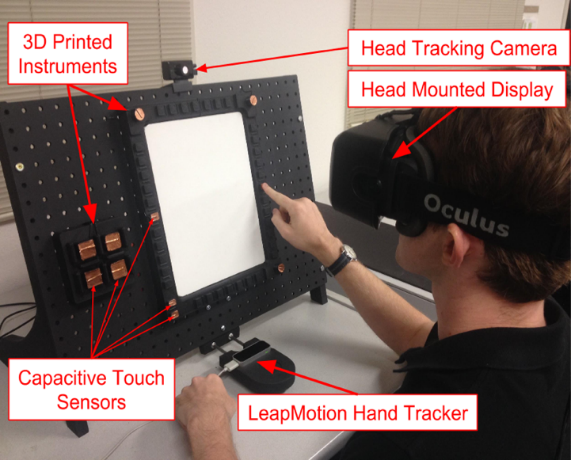
\includegraphics[width=.99\linewidth]{figures/r3c_callout.png}
    \caption{Subject using the system with major components annotated.}
    \label{fig:r3c_sub1}
  \end{subfigure}
  \begin{subfigure}{.49\textwidth}
    \centering
    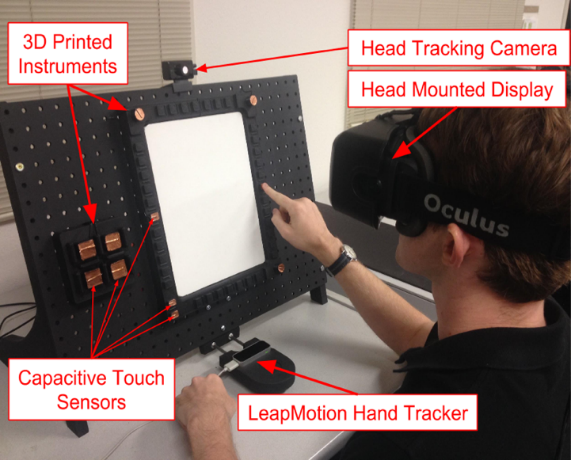
\includegraphics[width=.99\linewidth]{figures/r3c_callout.png}
    \caption{View presented to the user in the virtual world.}
    \label{fig:r3c_sub2}
  \end{subfigure}
  \caption{Rapidly Reconfigurable Research Cockpit}
\end{figure}

The VR head-mounted display (HMD) provides a virtual view of the cockpit environment.
A challenging aspect of immersive VR simula this, however, is to provide appropriate tactile feel of the objects being interacted with (in this case, the instruments of a cockpit).
We solve this by using 3D-printed instruments co-located with the virtual environment, which is a technique commonly called ``passive haptics''.
The instruments remain inert and non-functioning in the real world, but appear fully functional in the virtual world presented to the user.
The user can interact with the virtual cockpit (i.e.\ pressing buttons) with the use of the optical based hand tracker, which measures the position of the users hands.
This position is used to determine if the user is activating a button.
Measurements from the hand to display the essential visual feedback of hand position in the virtual world, as normally the use of an HMD blocks the view of ones own limbs.

\section{Background}
\subsection{Fitts' Law}
One of the most well studied relationships for human-computer input is Fitts Law\cite{fitts}.
Fitts' Law states that the movement time of human targeting motion is related to the size of the target (W) and the distance to the target (D).
These two geometrical parameters are combined in the index of difficulty (ID), which is presented here in the popular Shannons Formulation\cite{shannons}:
\begin{equation}
  ID=\log_2\left(\frac{D}{W}+1\right)
\end{equation}
The index of difficulty is linearly proportional to the movement time (MT), which provides the Fitts Law relationship:
\begin{equation}
  MT=a+b \cdot ID
\end{equation}
When comparing experimental conditions, it is recommended to use the measure of throughput (TP)\cite{four}.
This provides a single measure that encompasses speed and accuracy, averaging over the range of indices of difficulty.
Throughput has the units of bits per second, analogous to the amount of information, and is defined as the index of difficulty over the movement time:
\begin{equation}
  TP=\frac{ID}{MT}
\end{equation}
In studies of Fitts Law in which subjects are performing the task in two dimensions the ISO9421-9 circle multidirectional tapping task has become the standard\cite{five}.
A diagram of the task is shown in Figure~\ref{fig:circle}.

\begin{figure}[htb]
  \centering
  
\includegraphics[width=0.45\textwidth]{figures/iso9241.png}
  \caption{ISO9241 Fitts' Circle or multidirectional tapping task. D = distance, W = width.}
  \label{fig:circle}
\end{figure}

Fitts Law has been used in evaluating virtual environments and their input devices.
Chun et al.\cite{chun} evaluated a set of 3D stereo displays with a single haptic-enabled stylus using a Fitts tapping task.
Teather \& Stuerzlinger\cite{teather} performed a fully 3D targeting task using a hand tracker.
Liu et al.\cite{liu} performed a planar multi-directional Fitts task with a stereoscopic display, and compared virtual world to real world results, finding movement time twice as long in the virtual condition.
Kohli et al.\cite{kohli} evaluated passive haptics with warped virtual space to fool the user of the nature of the physical world.
They had the subjects perform an ISO9241-9 Fitts circle on a panel placed in front of them, and in some conditions the panel was rotated in the virtual world but not in the real world to create the discrepancy.
The subjects hand movement was warped to compensate for this.
Seixas et al.\cite{seixas} performed an ISO 9241-9 Fitts circle task with the same LeapMotion hand tracker we use, but did not employ any haptic feedback.

\subsection{Passive Haptics}
A constant challenge of virtual environments has been presenting the user with a tactile sensory input that matches the visual sensory inputs they are experiencing.
The focus of this work is the idea of passive haptics, whereby we recreate the tactile environment to provide the sense of touch and external forces.
The disadvantage is that the tactile environment cannot dynamically change during the simulation.
Fortunately, the adaptability (during simulation) of the passive haptic environment is not a requirement for the use case of aerospace cockpit simulation.
We still retain the ability to quickly change the environment via 3D printing new parts in between simulation sessions.

Schiefele et al.\cite{shiefele} used a head-mounted display (HMD) to replace the visuals of a flight simulator (though technology has drastically changed in HMDs and hand tracking since their publication).
They recreated only the positions of the panels with a flat plate and then used a magnetic hand tracker for reading the pilot input.
A short usability study was presented, and they found that users could activate switches, knobs and dials in less time with the physical panel than without (i.e.\ reaching into mid-air), a result reproduced here.
Insko\cite{insko} investigated the impact of passive haptics on generic virtual environments.
It was found that the passive haptics increased the sense of presence felt by users.
An experiment had two groups complete a maze in a virtual environment, one group with passive haptics on boundaries, and one without.
After training the passive haptic group bumped into far fewer obstacles than the group without.
Borst and Volz\cite{borst} created a ``mixed'' haptic virtual environment, whereby they combined an active haptic glove with a passive haptic panel.
They found the glove by itself consistently performed worse than the other two, but overall no significant difference existed between passive haptics and their mixed haptics, again indicating the power of simple passive haptics.

\section{Methods}
\subsection{Technical Approach}
The head mounted display used is an Oculus Rift Development Kit 2.
The hand tracker, LeapMotion, is mounted above and pointed down so the field of view encompasses the area in front of the panel.
A custom calibration program is run to line up the LeapMotion measurements with the virtual world in the rendering engine.
For the experiment reported here, a blank panel (45cm x 45cm) was used to provide only the backstop of the virtual buttons for the ``Passive Haptics'' condition.
Subjects were seated in front of the panel.
The button selection is registered by the subject moving their index finger into a hover zone (cylinder for the circle buttons) in front of the button that extends outward 1.27cm.
Their entrance into the hover zone is indicated to them by the button changing color.
A successful button press is registered after 160ms, and is indicated by the color turning off and a button click noise being played over speakers.

The authors previous study\cite{r3c} asked subjects to complete a discrete button targeting task, and validated our technical approach.
Subjects were able to select the buttons in the virtual world as accurately as in the real world, albeit with a small time penalty, consistent with other studies comparing real world to virtual world inputs\cite{eight}.
However, the difference between the passive haptic and no passive haptic condition was insignificant, leading to a more extensive Fitts evaluation that is presented in this paper.
The experimental setup for this study consisted of two conditions, one with the panel (``Passive Haptics'') and one without the panel (``No Passive Haptics''), where the subjects would need to target the buttons in mid-air.
The different conditions and the view of the virtual world is shown in Figure 3.

\begin{figure}[tb]
  \centering
  \begin{subfigure}{.32\textwidth}
    \centering
    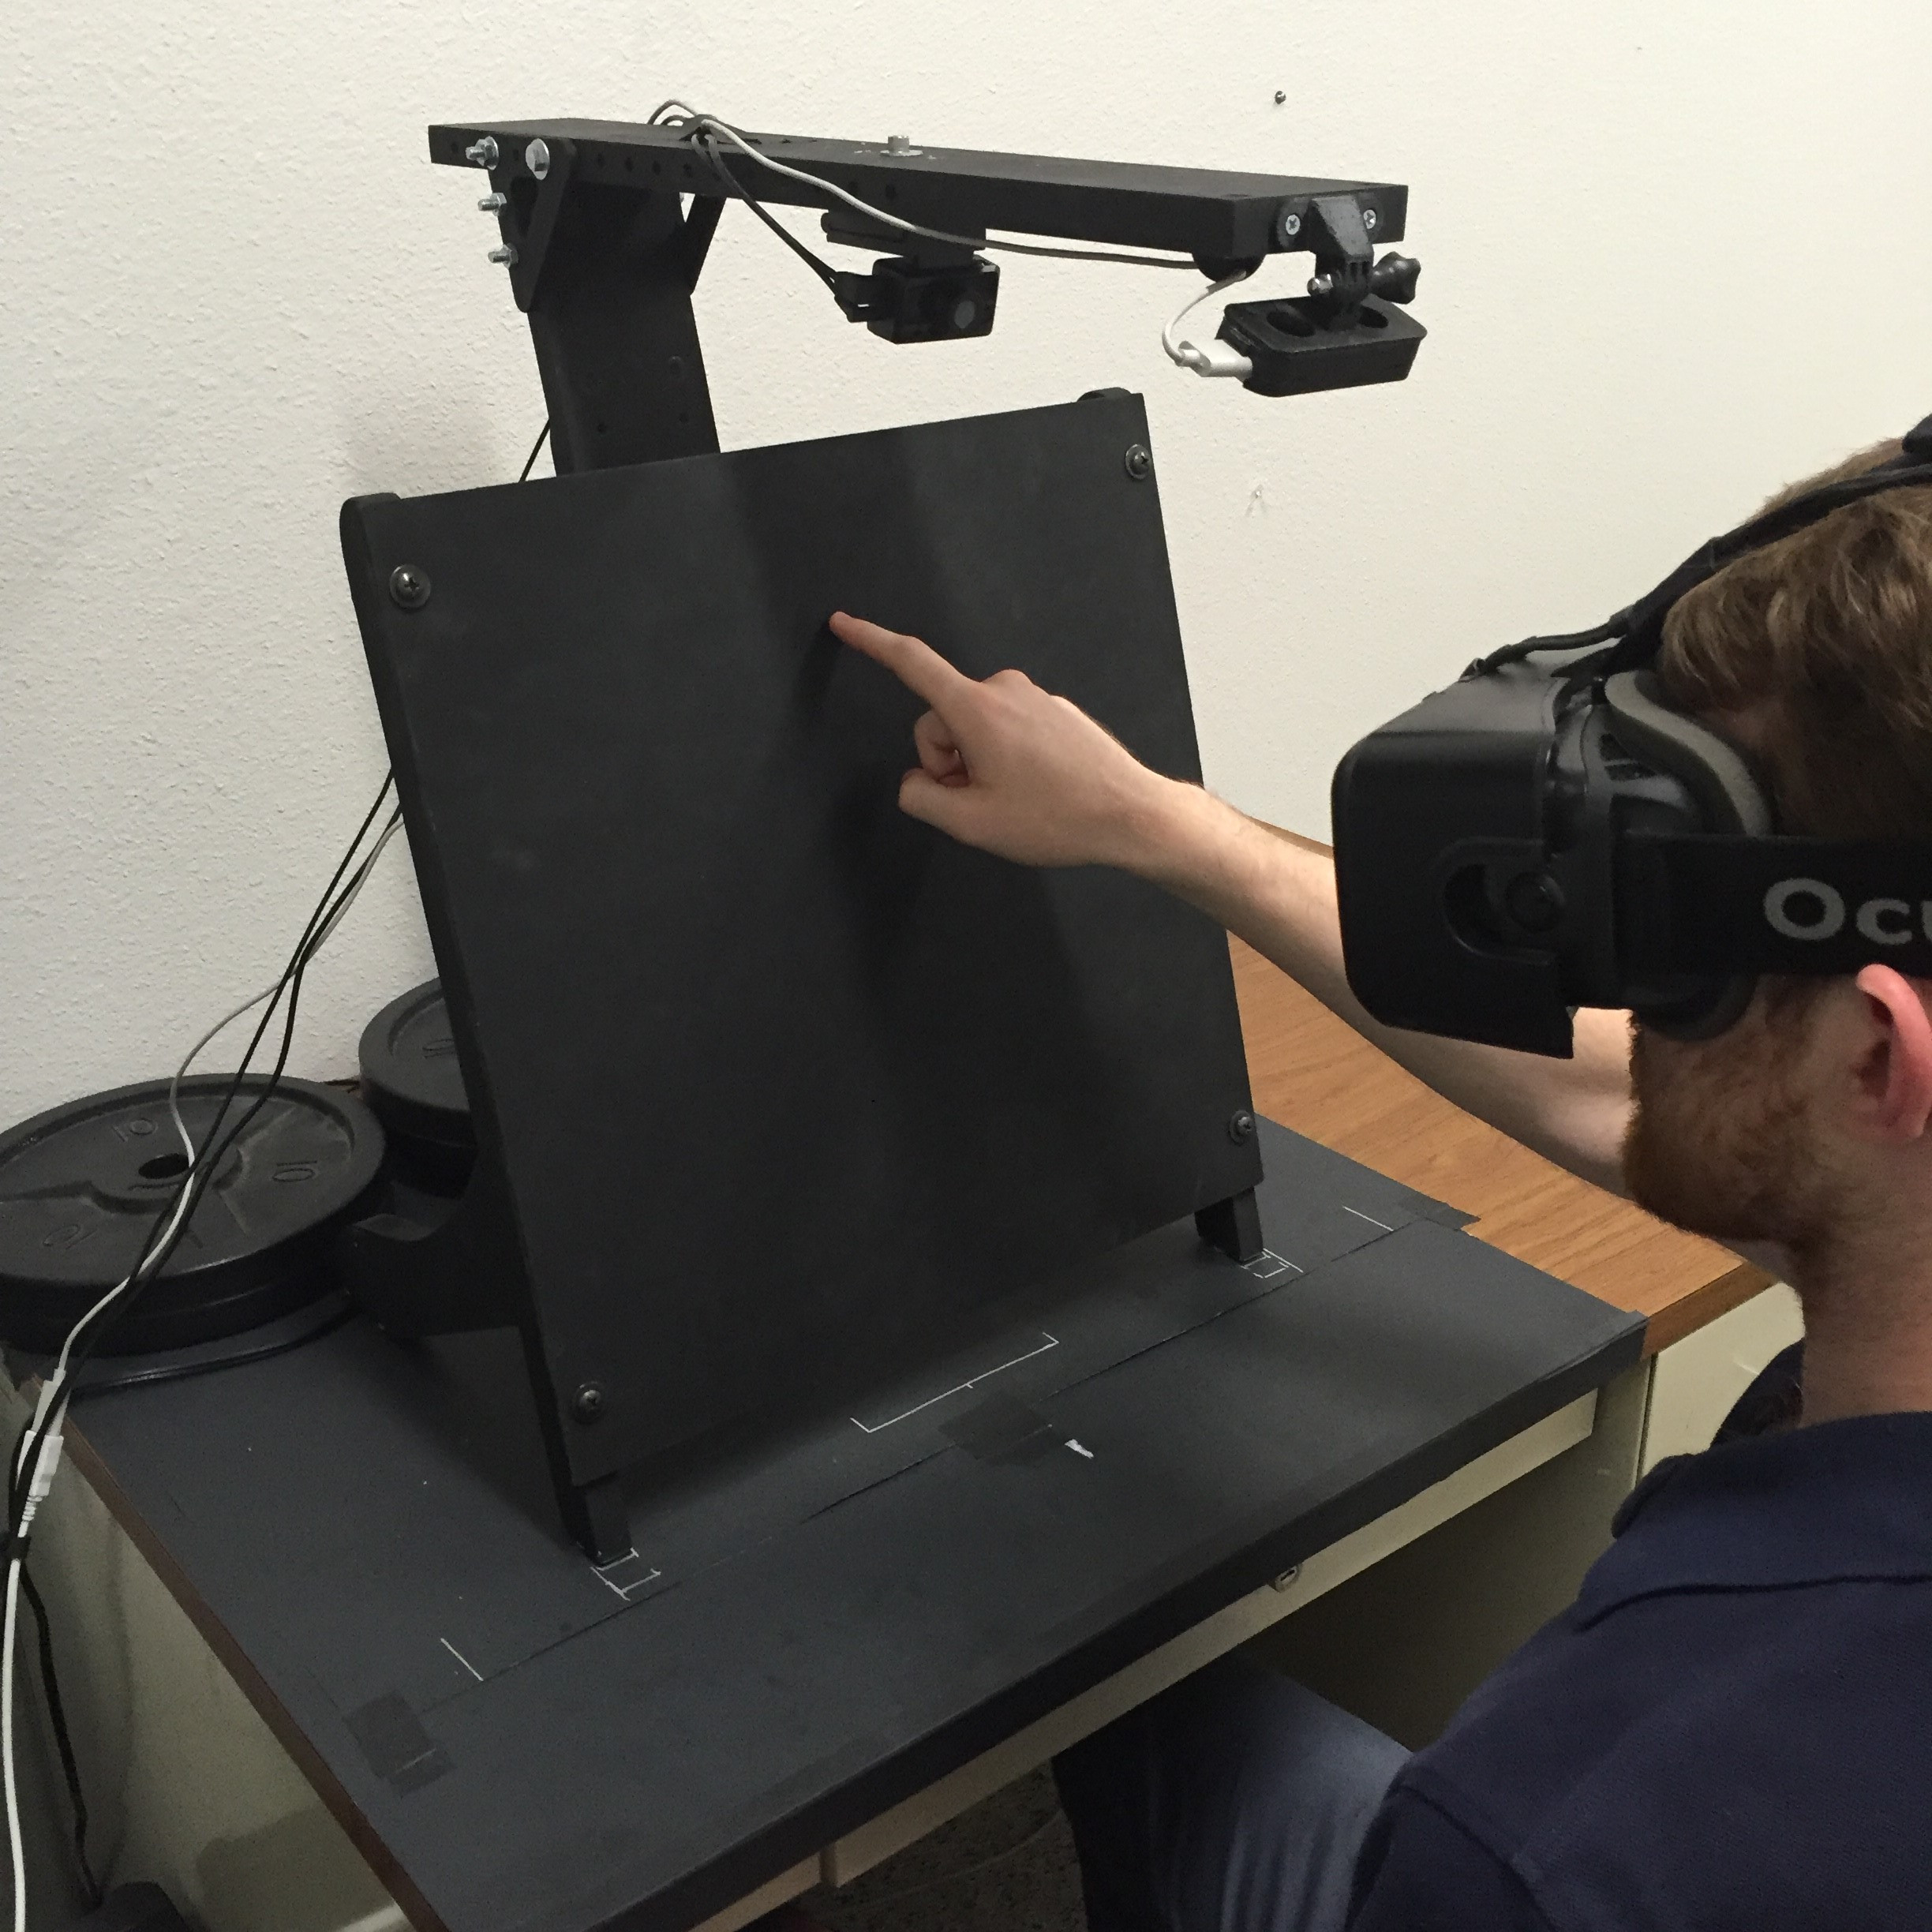
\includegraphics[width=.99\linewidth]{figures/passive_haptics.jpg}
    \caption{\textit{Passive Haptics} condition}
    \label{fig:passive_haptics}
  \end{subfigure}
  \begin{subfigure}{.32\textwidth}
    \centering
    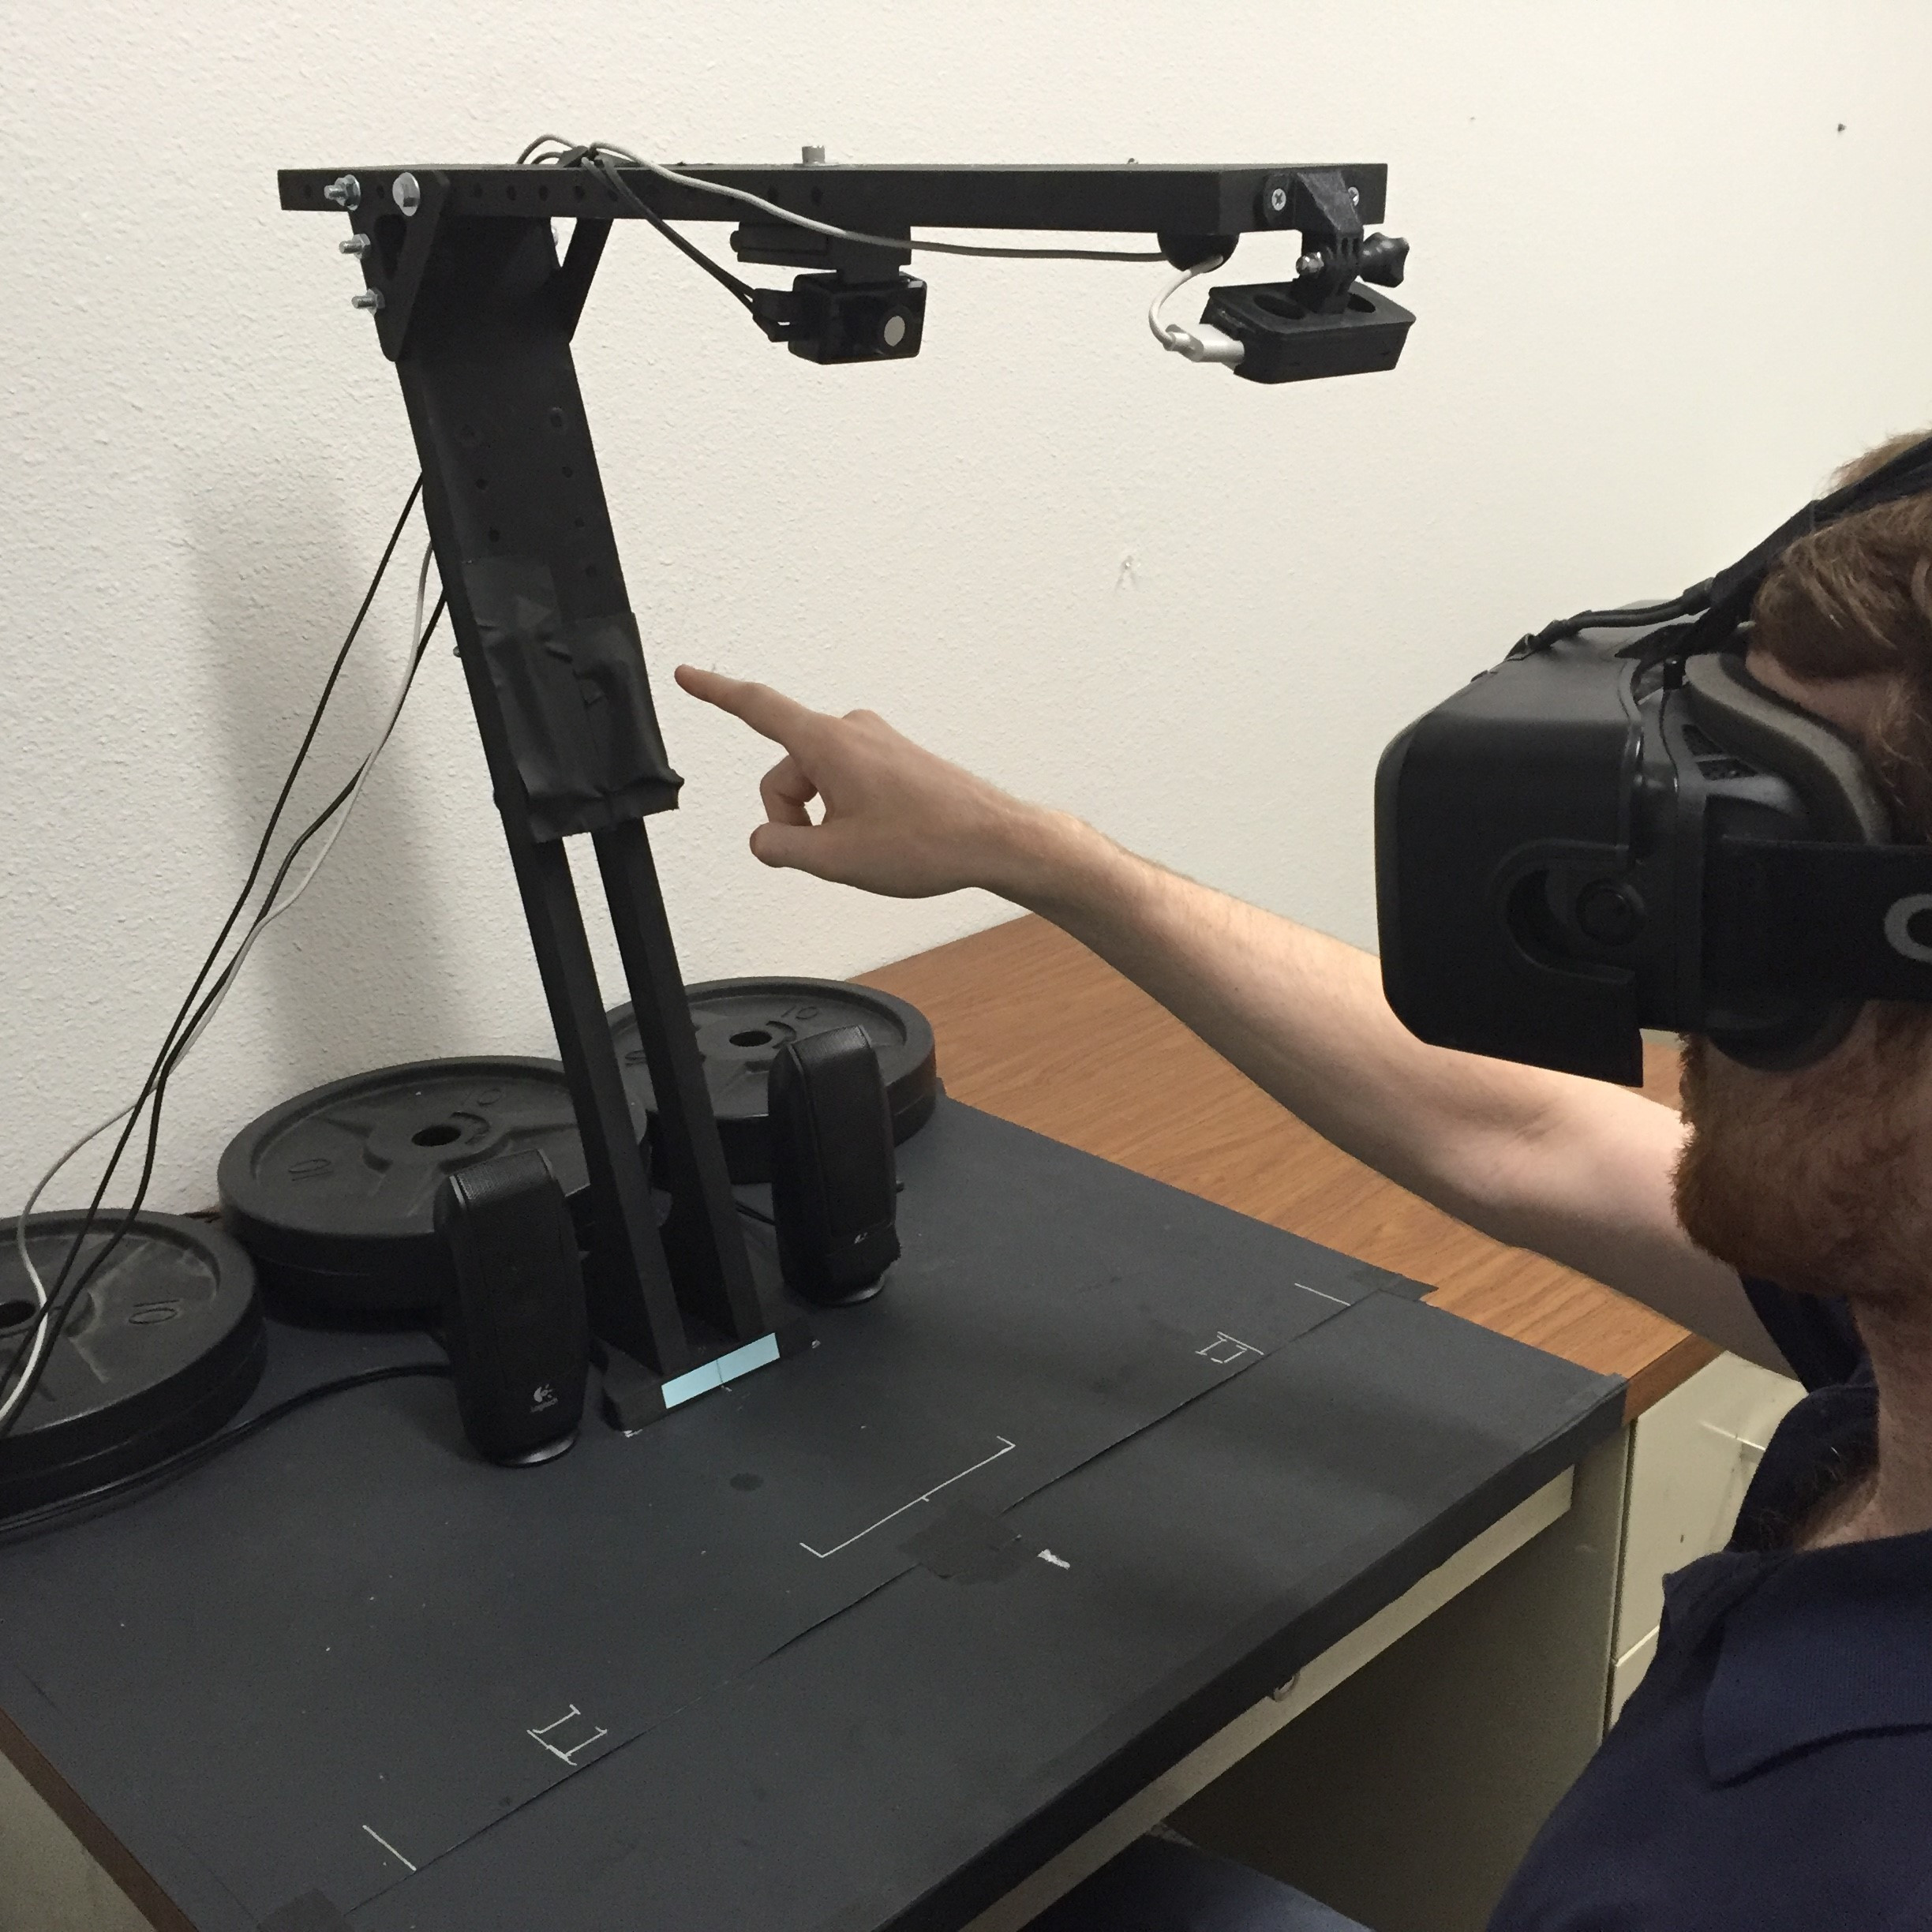
\includegraphics[width=.99\linewidth]{figures/no_passive_haptics.jpg}
    \caption{\textit{No Passive Haptics} condition}
    \label{fig:no_passive_haptics}
  \end{subfigure}
  \begin{subfigure}{.32\textwidth}
    \centering
    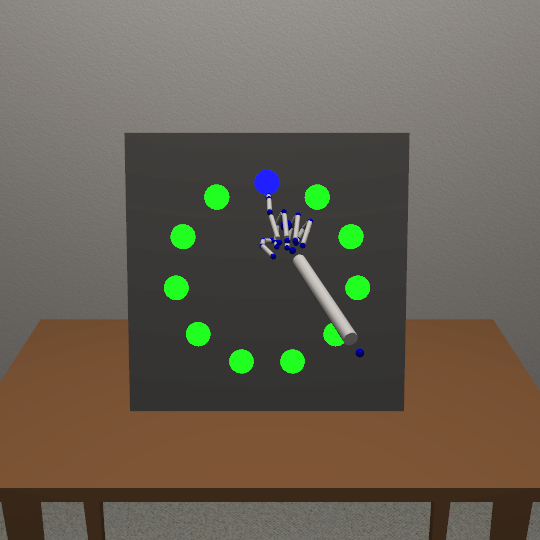
\includegraphics[width=.99\linewidth]{figures/virtual_view.png}
    \caption{Virtual world view}
    \label{fig:virtual_view}
  \end{subfigure}
  \caption{Experimental Setup}
\end{figure}

\subsection{Experimental Task}
Subjects were asked to complete 15 configurations of the Fitts ISO9241-9 circle, as shown in Figure 2.
The configurations comprised of 3 distances (D) of 20cm, 30cm and 40cm and 5 widths (W) ranging from 5mm to 25mm in 5mm increments.
Every circle contained 11 targets.
They performed each circle sequence three times in a row before proceeding to the next configuration.
The target width order was chosen randomly, but the order of the distances was sequenced from smallest to largest for half of the subjects, and largest to smallest for the other half.

The 15 circle configurations were completed for each subject in both conditions, with passive haptics and without passive haptics.
The order of the conditions was counterbalanced so that half saw the passive haptic condition first.
Subjects were not instructed on the second condition before they finished the first condition (i.e.\ subjects who started with no passive haptics were not told the second half would proceed with a passive haptic in place, and could not see the real panel in the experimental room).
At the conclusion of each condition, they were given a presence questionnaire of 21 questions on a 7 point Likert scale, with questions from the Presence Questionnaire and Slater-Usoh-Steed questionnaire.
At the conclusion of the experiment, a condition comparison questionnaire was administered to directly compare subjects perceptions of the two conditions, with a 7 point Likert scale anchored from ``With Panel'' to ``Without Panel''.
The subjects were asked after every other circle completion to provide an arm fatigue rating based on the Borg RPE (Rating of Perceived Exertion) scale (between 6-20).

\section{Results \& Discussion}
Twenty (20) subjects performed the experiment, all engineering students (undergraduate and graduate).
All subjects had less than an hour experience with virtual reality devices, with half indicating no previous experience.
Subjects used their dominant hand index finger to target the buttons.
In order to compensate for the training effects, we present the Fitts Law results for the middle circle (D=30cm) as all subjects in all conditions performed this circle configuration second.
Including all results does not significantly change the Fitts parameters (and in fact artificially inflates the difference as subjects take longer to learn in the No Passive Haptics condition).
The regression plot is shown in Figure 4, and the parameters are listed in Table 1, along with the throughput calculation.
The throughput of each condition is calculated as a mean-of-means, whereby first a mean for each index of difficultly for each subject is found, before averaging between subjects.

The amount of time taken to complete the entire condition (15 circle configurations) is shown in Table 2.
Half of the subjects performed the Passive Haptics condition first followed by the No Haptics condition, while the other half did the reverse.
Overall, subjects were able to complete the passive haptics condition much faster (13.3 minutes to 17.1 minutes, respectively).
The subjects who started with passive haptics were then able to complete the no haptics condition almost 3 minutes faster (16\%) than those who started with no haptics, compared to less than a minute improvement for the other subject group (7\%).
This indicates that the passive haptics provides more transfer of training, or the penalty for learning the virtual environment is less with passive haptics.
There was no significant difference of the scores of the presence questionnaire between conditions.
The self-reported arm fatigue shows that subjects who start with No Haptics end the first condition with a higher arm fatigue, but as shown in Table 2, the subjects also took more time to complete that condition, so it is unclear if the cause of the fatigue is the lack of panel or simply accumulation of time.
The results from the condition comparison survey are shown in Figure 5.
Most subjects preferred the Passive Haptics condition, with only 2 indicating no preference.
Similar results were found when asking the subjects if they felt they performed faster or more accurately in one condition or the other, with the vast majority indicating they felt faster and more accurate in the Passive Haptics condition.
Most subjects felt that they fatigued more or quicker in the No Haptics condition, but this was not as heavily weighted to one side of the scale as the other results.


\section{Conclusion}
We evaluated a hand-tracked, passive haptic interface for virtual reality head mounted displays using a Fitts ISO9241-9 multidirectional tapping task.
We found increased Fitts throughput when subjects had a physical panel (passive haptics) in position with the virtual buttons than without a physical panel.
Subjects were able to train quicker in the virtual environment with the passive haptics than without.
Subjects perceived that they performed faster and more accurately with the passive haptics, and overall preferred the passive haptic condition.



% produces the bibliography section when processed by BibTeX
% \nocite{*}
%\bibliography{bibtex_database}
%\bibliographystyle{aiaa}

\end{document}

% - Release $Name:  $ -
